\documentclass[12pt]{beamer}

\usepackage[T1]{fontenc}
\usepackage[utf8]{inputenc}
\usepackage[british]{babel}
\usepackage{mathtools}
\usepackage{amsthm}
\usepackage{libertine}
\usepackage[libertine]{newtxmath}
\usepackage[mathscr]{euscript}
\usepackage{tikz-cd}
\usepackage{tikz}
\usetikzlibrary{decorations.markings}
\usepackage{float}
\usepackage[
  backend=biber,
  style=alphabetic,
  maxnames=10,
  maxalphanames=10]{biblatex}
\addbibresource{refs.bib}
\usepackage{hyperref}
\urlstyle{same}

\usefonttheme{serif}
\usetheme{Singapore}
\usecolortheme{rose}

\title[UPM ETSIT]{Diagonalización de endomorfismos: \\ Autovectores y autovalores}
\author{Pedro N\'{u}\~{n}ez}
\institute{Grado en Ingeniería de Tecnologías y Servicios de Telecomunicación \\ --- \\ Álgebra}
\date{\small 18 de mayo de 2026 \\ \vspace{4mm} UPM --- ETSIT}

\makeatletter
\hypersetup{
  pdftitle={@title},
  colorlinks,
  linkcolor=[rgb]{0.2,0.2,0.6},
  citecolor=[rgb]{0.2,0.6,0.2},
  urlcolor=[rgb]{0.6,0.2,0.2}}
\makeatother

% Comando personalizado para el QR
% #1: Ancho de la imagen
% #2: Opacidad (1.0 = Negro puro, 0.3 = Gris claro/Transparente)
\newcommand{\ponerQR}[2]{
    \begin{tikzpicture}[remember picture, overlay]
        % The opacity is now applied to the TikZ node, not \includegraphics
        \node[anchor=south east, inner sep=15pt, opacity=#2] at (current page.south east) {
            
\includegraphics[width=#1]{QR.png}
        };
    \end{tikzpicture}
}

% 1. Para que aparezca en todas las diapositivas de contenido (pequeño y gris)
\addtobeamertemplate{background}{\ponerQR{1.5cm}{0.3}}{}

\begin{document}

{
    % Sobrescribimos la plantilla solo para este bloque
    \setbeamertemplate{background}{\ponerQR{2.2cm}{1.0}}
    \begin{frame}[plain]
        \titlepage
    \end{frame}
}

\begin{frame}
  \frametitle{Ejemplo:~sucesiones recursivas}
  Sea
  \vspace{-8mm}
  \begin{align*}
    a_{0} & = 3 \\
    a_{1} & = 4 \\
    a_{2} & = 3a_{1} - 2a_{0} = 6 \\
     & \hspace{2mm} \vdots \\
    a_{n+1} & = 3a_{n} - 2a_{n-1}.
  \end{align*}
  \pause

  \textbf{Pregunta:}
  ¿Cuánto vale $a_{11}$?

\end{frame}

\begin{frame}
  \frametitle{Observación 1}
  Podemos reescribir esta sucesión con una matriz:
  \[
    \begin{pmatrix}
      a_{n+1} \\
      a_{n}
    \end{pmatrix}
    =
    \begin{pmatrix}
      3 & -2 \\
      1 & 0
    \end{pmatrix}
    \begin{pmatrix}
      a_{n} \\
      a_{n-1}
    \end{pmatrix}
  \]
  para todo $n > 0$.
  \pause

  \vspace{7mm}
  Sea $A :=
  \begin{pmatrix}
    3 & -2 \\
    1 & 0
  \end{pmatrix}$.
  Por inducción, vemos que
  \[ 
    \begin{pmatrix}
      a_{n+1} \\
      a_{n}
    \end{pmatrix}
    =
    A^{n}
    \begin{pmatrix}
      a_{1} \\
      a_{0}
    \end{pmatrix}
    =
    A^{n}
    \begin{pmatrix}
      4 \\
      3
    \end{pmatrix}.
  \]

\end{frame}

\begin{frame}
  \frametitle{Observación 1}
  Por lo tanto, podemos calcular $a_{11}$ de la siquiente manera:

  \[
    \begin{pmatrix}
      {\color{red}a_{11}} \\
      a_{10}
    \end{pmatrix}
    =
    A^{10}
    \begin{pmatrix}
      4 \\
      3
    \end{pmatrix}.
  \]
  \pause

  \vfill
  $\quad \rightsquigarrow$ Basta con calcular $A^{10}$.
\end{frame}

\begin{frame}
  \frametitle{Observación 2}
  La matriz $A$ es la representación matricial del endomorfismo
  \begin{align*}
    f \colon \mathbb{R}^{2} & \to \mathbb{R}^{2} \\
    (x,y) & \mapsto (3x-2y,x)
  \end{align*}
  respecto a la base canónica $\mathcal{E} = \{ (1,0), (0,1) \}$ de $\mathbb{R}^{2}$.
  \pause

  Es decir,
  \[
    A = M_{\mathcal{E}}(f).
  \]
  \pause

  $\quad \rightsquigarrow$ Basta con calcular el endomorfismo $f \circ \overset{10)}{\cdots} \circ f$, \\
  porque
  \[
    A^{10}
    \begin{pmatrix}
      4 \\
      3
    \end{pmatrix}
    = [(f \circ \overset{10)}{\cdots} \circ f)(4,3)]_{\mathcal{E}}.
  \]

\end{frame}


\begin{frame}
  \frametitle{Elegir una base apropiada}
  La aplicación lineal $g := f \circ \overset{10)}{\cdots} \circ f$ está completamente determinada por la imagen de los vectores de una base.
  \pause

  \vspace{5mm}
  $\quad \rightsquigarrow$ Podemos usar la base de $\mathbb{R}^{2}$ que más nos convenga para calcular $g$.
  \pause
  
  \vspace{5mm}
  \textbf{Pregunta:}
  ¿Existe una base $\mathcal{B} = \{ v_{1}, v_{2} \}$ de $\mathbb{R}^{2}$ tal que las imágenes de $g(v_{1})$ y $g(v_{2})$ sean fáciles de calcular?
  
    
\end{frame}

\begin{frame}
  \frametitle{Elegir una base apropiada}
  Por ejemplo, $f(1,0) = (3,1)$.
  \begin{center}
    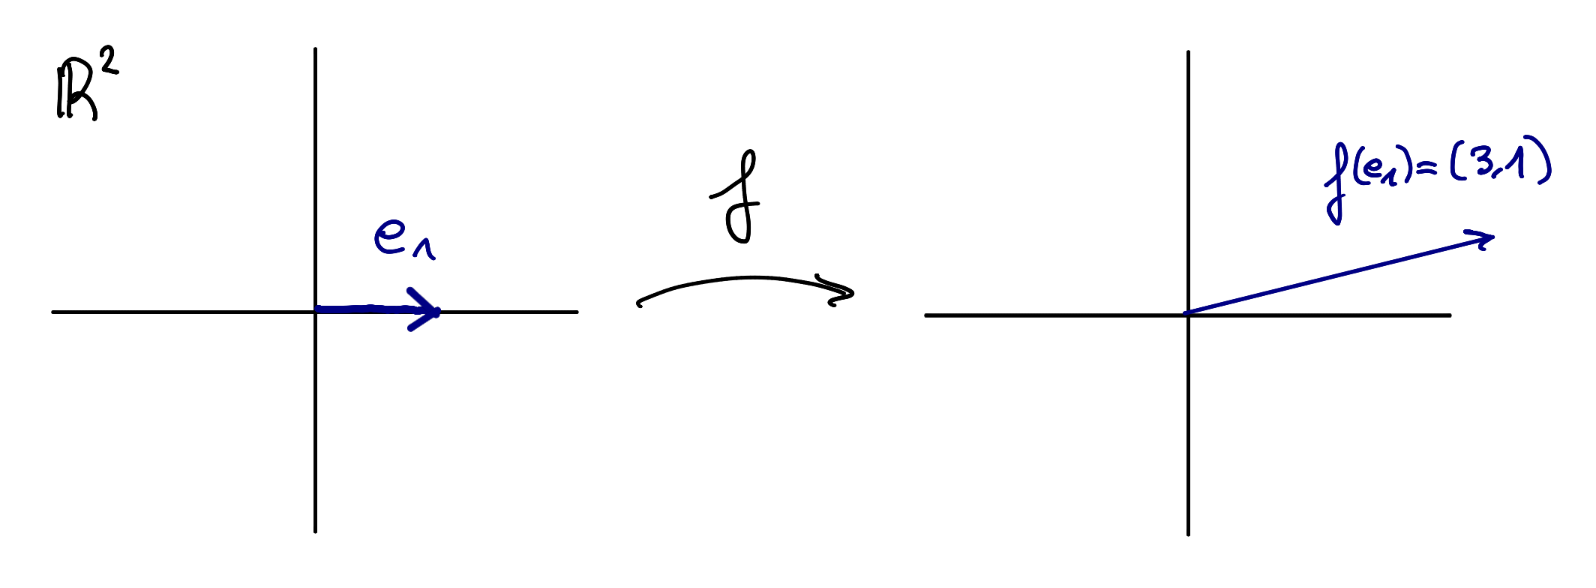
\includegraphics[scale=.15]{linear-map-1.png}
  \end{center}
  \pause

  $\quad \rightsquigarrow$ No es fácil calcular $g(1,0)$.

\end{frame}

\begin{frame}
  \frametitle{Elegir una base apropiada}
  En cambio, para $v_{1} = (1,1)$, tenemos que $f(1,1) = (1,1)$.
  \begin{center}
    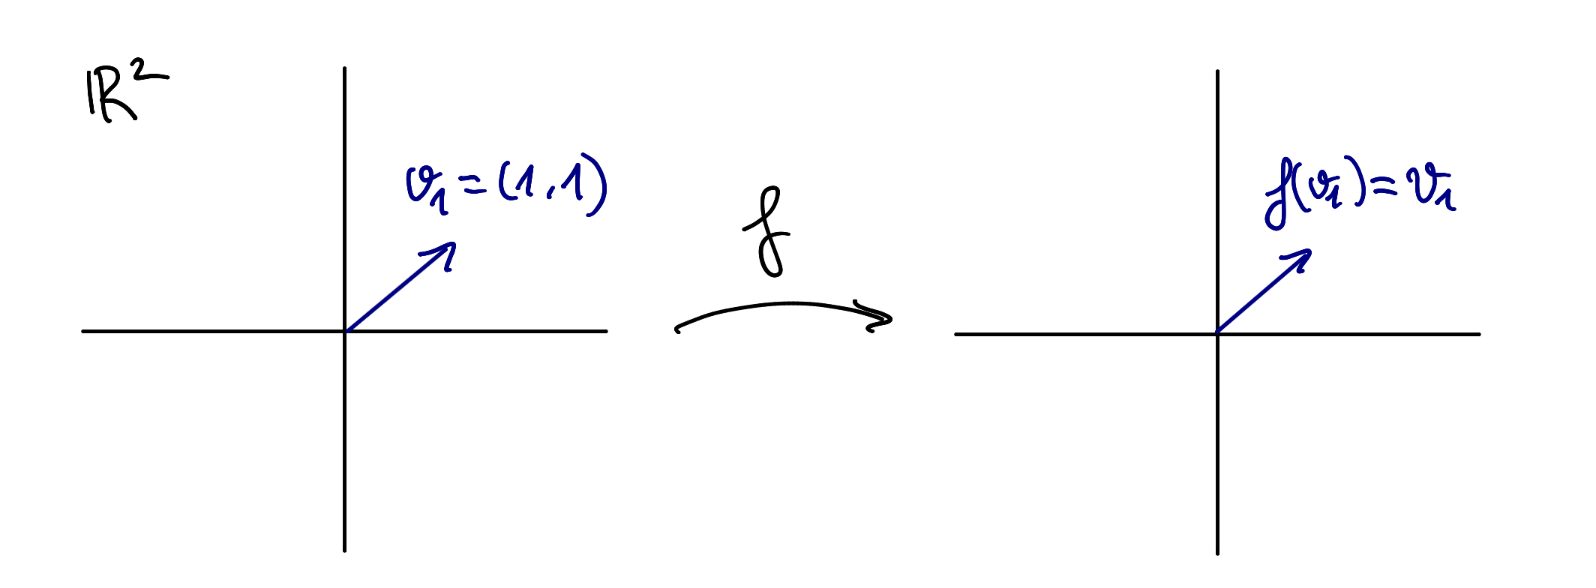
\includegraphics[scale=.15]{linear-map-2.png}
  \end{center}
  \pause

  $\quad \rightsquigarrow$ Es fácil calcular $g(1,1)$:
  \[ g(1,1) = f \circ \overset{10)}{\cdots} \circ f(1,1) = (1,1). \]

\end{frame}

\begin{frame}
  \frametitle{Elegir una base apropiada}
  Para $v_{2} = (2,1)$, tenemos que
  \[ f(2,1) = (4,2) = {\color{red} 2}\cdot (2,1). \]

  \begin{center}
    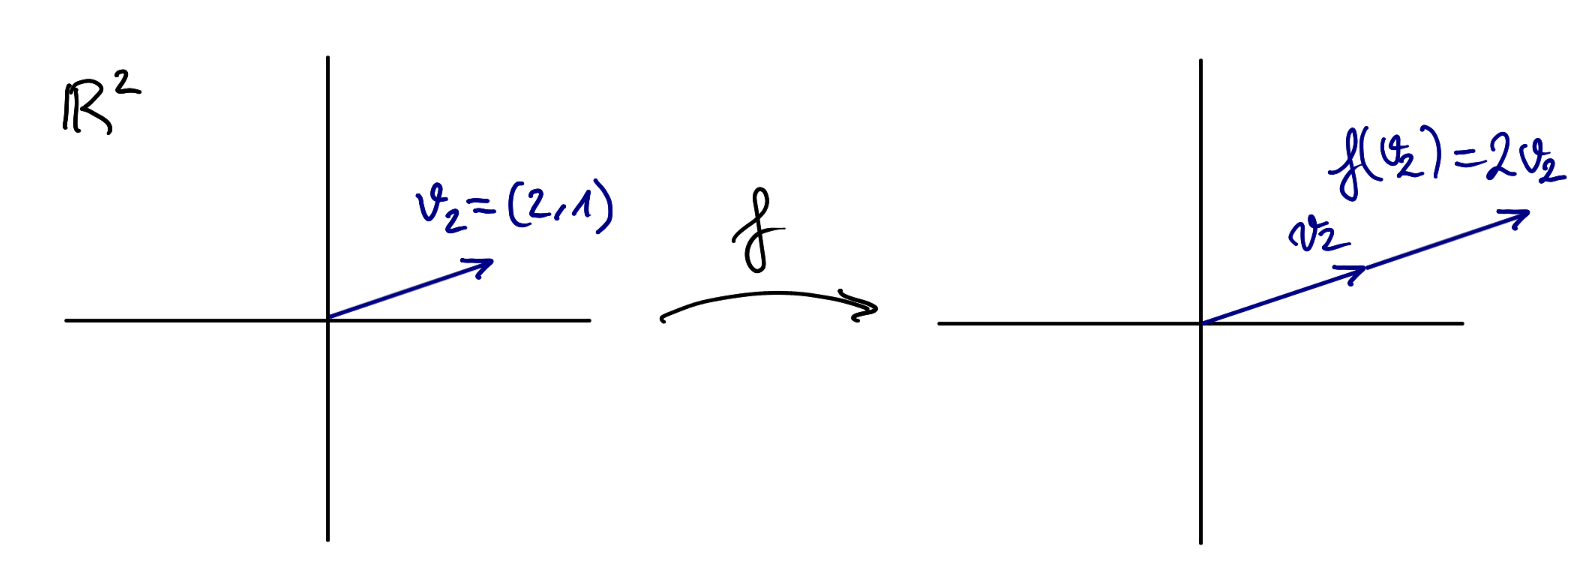
\includegraphics[scale=.15]{linear-map-3.png}
  \end{center}
  \pause

  $\quad \rightsquigarrow$ Es fácil calcular $g(2,1)$:
  \[ g(2,1) = f \circ \overset{10)}{\cdots} \circ f(2,1) = 2^{10}\cdot (2,1). \]

\end{frame}

\begin{frame}
  \frametitle{Elegir una base apropiada}
  Es decir, respecto a la base $\mathcal{B} = \{ v_{1}, v_{2} \}$,
  la matriz representante de $f$ es la matriz diagonal
  \[
    M_{\mathcal{B}}(f) =
    \begin{pmatrix}
      1 & 0 \\
      0 & 2
    \end{pmatrix},
  \]
  \pause
  y la matriz representente de $g$ es
  \[
    M_{\mathcal{B}}(g) = M_{\mathcal{B}}(f)^{10} =
    \begin{pmatrix}
      1^{10} & 0 \\
      0 & 2^{10}
    \end{pmatrix}
    =
    \begin{pmatrix}
      1 & 0 \\
      0 & 1024
    \end{pmatrix}
  \]

\end{frame}

\begin{frame}
  \frametitle{Elegir una base apropiada}
  \begin{itemize}
    \item Los vectores $v_{1}$ y $v_{2}$ satisfacen que su imagen por $f$ es un \textbf{múltiplo escalar} del mismo vector, y esto nos permite obtener una matriz representante de $f$ \textbf{diagonal}.
      \pause
      \vspace{5mm}
    \item \textit{(Spoiler)} Este tipo de vectores se llaman \textbf{autovectores} de $f$,
  y el proceso de hallar una base respecto de la cual la matriz de $f$ sea diagonal se llama \textbf{diagonalización} del endomorfismo $f$.
  \end{itemize}

\end{frame}

\begin{frame}
  \frametitle{Conclusión del ejemplo}
  Como $(4,3) = 2 \cdot (1,1) + 1 \cdot (2,1)$,
  tenemos que
  \[
    [(4,3)]_{\mathcal{B}} =
    \begin{pmatrix}
      2 \\
      1
    \end{pmatrix}.
  \]
  Por lo que hemos visto antes,
  y por definición de matriz representante,
  tenemos que
  \[
    [g(4,3)]_{\mathcal{B}} =
    \begin{pmatrix}
      1 & 0 \\
      0 & 1024
    \end{pmatrix}
    \begin{pmatrix}
      2 \\
      1
    \end{pmatrix}
    =
    \begin{pmatrix}
      2 \\
      1024
    \end{pmatrix}.
  \]

\end{frame}

\begin{frame}
  \frametitle{Conclusión del ejemplo}
  Por definición,
  \[
    [g(4,3)]_{\mathcal{B}} =
    \begin{pmatrix}
      2 \\
      1024
    \end{pmatrix}
  \]
  quiere decir que
  \begin{align*}
    g(4,3) & = 2 \cdot (1,1) + 1024 \cdot (2,1) \\
    & = (2050, 1026).
  \end{align*}
  \pause
  Por lo tanto, como $(a_{11},a_{10}) = g(4,3)$,
  deducimos finalmente que
  \[
    a_{11} = 2050.
  \]

\end{frame}

\begin{frame}
  \frametitle{Definición: autovector y autovalor}
  Sea $V$ un espacio vectorial y sea $f \colon V \to V$ un endomorfismo.
  \pause
  \begin{itemize}
    \item Un vector $v \in V$ {\color{red} no nulo} se llama \textbf{autovector} de $f$ si existe un escalar $\lambda$ tal que
      \[ f(v) = \lambda \cdot v. \]
      \pause
      \vspace{-8mm}
    \item Un escalar $\lambda$ como en el punto anterior se llama \textbf{autovalor} de $f$.
      \pause
    \item En la situación anterior,
      diremos que $v$ es un autovector correspondiente al autovalor $\lambda$.
  \end{itemize}

\end{frame}

\begin{frame}
  \frametitle{Autovectores y autovalores}
  \vspace{-8mm}
  \begin{itemize}
    \item En la definición anterior, es importante darse cuenta de que los autovectores son no nulos por definición, pero los autovalores pueden ser nulos.
      \pause
    \item En la práctica hablaremos de autovectores y autovalores de una matriz cuadrada $A$.
      Nos referimos a los autovalores y autovectores del endomorfismo $f \colon \mathbb{R}^{n} \to \mathbb{R}^{n}$ tal que $M_{\mathcal{E}}(f) = A$.
      \pause
    \item El escalar $0$ es un autovalor de una matriz cuadrada $A$ \\
      si y solo si $\det(A) = 0$.
  \end{itemize}
\end{frame}


\begin{frame}
  \frametitle{Definición: diagonalización de un endomorfismo}
  Sea $V$ un espacio vectorial y sea $f \colon V \to V$ un endomorfismo.
  \pause
  \begin{itemize}
    \item \textbf{Diagonalizar} el endomorfismo $f$ consiste en encontrar una base $\mathcal{B}$ de $V$ tal que $M_{\mathcal{B}}(f)$ sea diagonal:
      \[
        M_{\mathcal{B}}(f) =
        \begin{pmatrix}
          \lambda_{1} & 0 & \cdots & 0 \\
          0 & \lambda_{2} & \cdots & 0 \\
          \vdots & \vdots &  & \vdots \\
          0 & 0 & \cdots & \lambda_{n}
        \end{pmatrix}.
      \]
      \pause
    \item Equivalentemente, consiste en encontrar una base \\
      de $V$ de autovectores de $f$.
  \end{itemize}
\end{frame}

\begin{frame}
  \frametitle{Diagonalización de una matriz}
  \begin{itemize}
    \item En la práctica, igual que hablamos de autovalores y autovectores de una matriz $A$, hablaremos de diagonalizar una matriz $A$.
    Esto quiere decir encontrar una matriz invertible $P$ tal que
    \[ 
      P^{-1} A P = D
    \]
    sea diagonal.
    \pause
  \item En el caso de que $A$ sea diagonalizable, podemos obtener $P$ como la matriz cuyas columnas son los vectores \\
    de una base de autovectores.
  \end{itemize}

\end{frame}

\begin{frame}
  \frametitle{¿Son todos los endomorfismos diagonalizables?}

  \textbf{Deberes:}
  Da un ejemplo de un endommorfismo $f$ de $\mathbb{R}^{2}$ que no tenga ningún autovector.
  Explica con palabras por qué esto implica que $f$ no es diagonalizable.

\end{frame}


{
    % Sobrescribimos la plantilla solo para este bloque
    \setbeamertemplate{background}{\ponerQR{2.2cm}{1.0}}
    \begin{frame}[plain]
      \vfill
      \begin{center}
        \usebeamercolor[fg]{frametitle}
        \usebeamerfont{frametitle}
        ¡Gracias por vuestra atención!
      \end{center}
      \vfill
    \end{frame}
}


\end{document}
